\documentclass[fleqn]{thesis}

% DOCUMENT
\usepackage{kantlipsum}

\graphicspath{{./ch3_creteil/img/}{./ch2_gridshell/img/}}


\begin{document}

	\part{My First Part}
		\chapter{Mon premier chapitre}
		\section{Une section}
		\kant[1-4]
		\section{Une deuxième section}
		\kant[1-2]
		\section{Une troisième section}
		\kant[1-2]
	
	\part{My Second Part}
		% \chapter{Mon premier chapitre}
		% \section{Une section}
		% \kant[1-20]
		% \section{Une deuxième section}
		% \kant[1-2]
		% \section{Une troisième section}
		% \kant[1-2]
		\cref{fig:twospread}


	\def\mycap{
		% \begin{textblock*}{5cm}(1cm,1cm)
		% 	\raggedright
		% 	\captionof{figure}{\LARGE\bfseries\color{white}sdsdksdmskdms\label{fig:twospread}}
		% \end{textblock*}
	}

	\clearpage
	% \begin{textblock*}{0.5\paperwidth}(0cm,0cm)
	% 	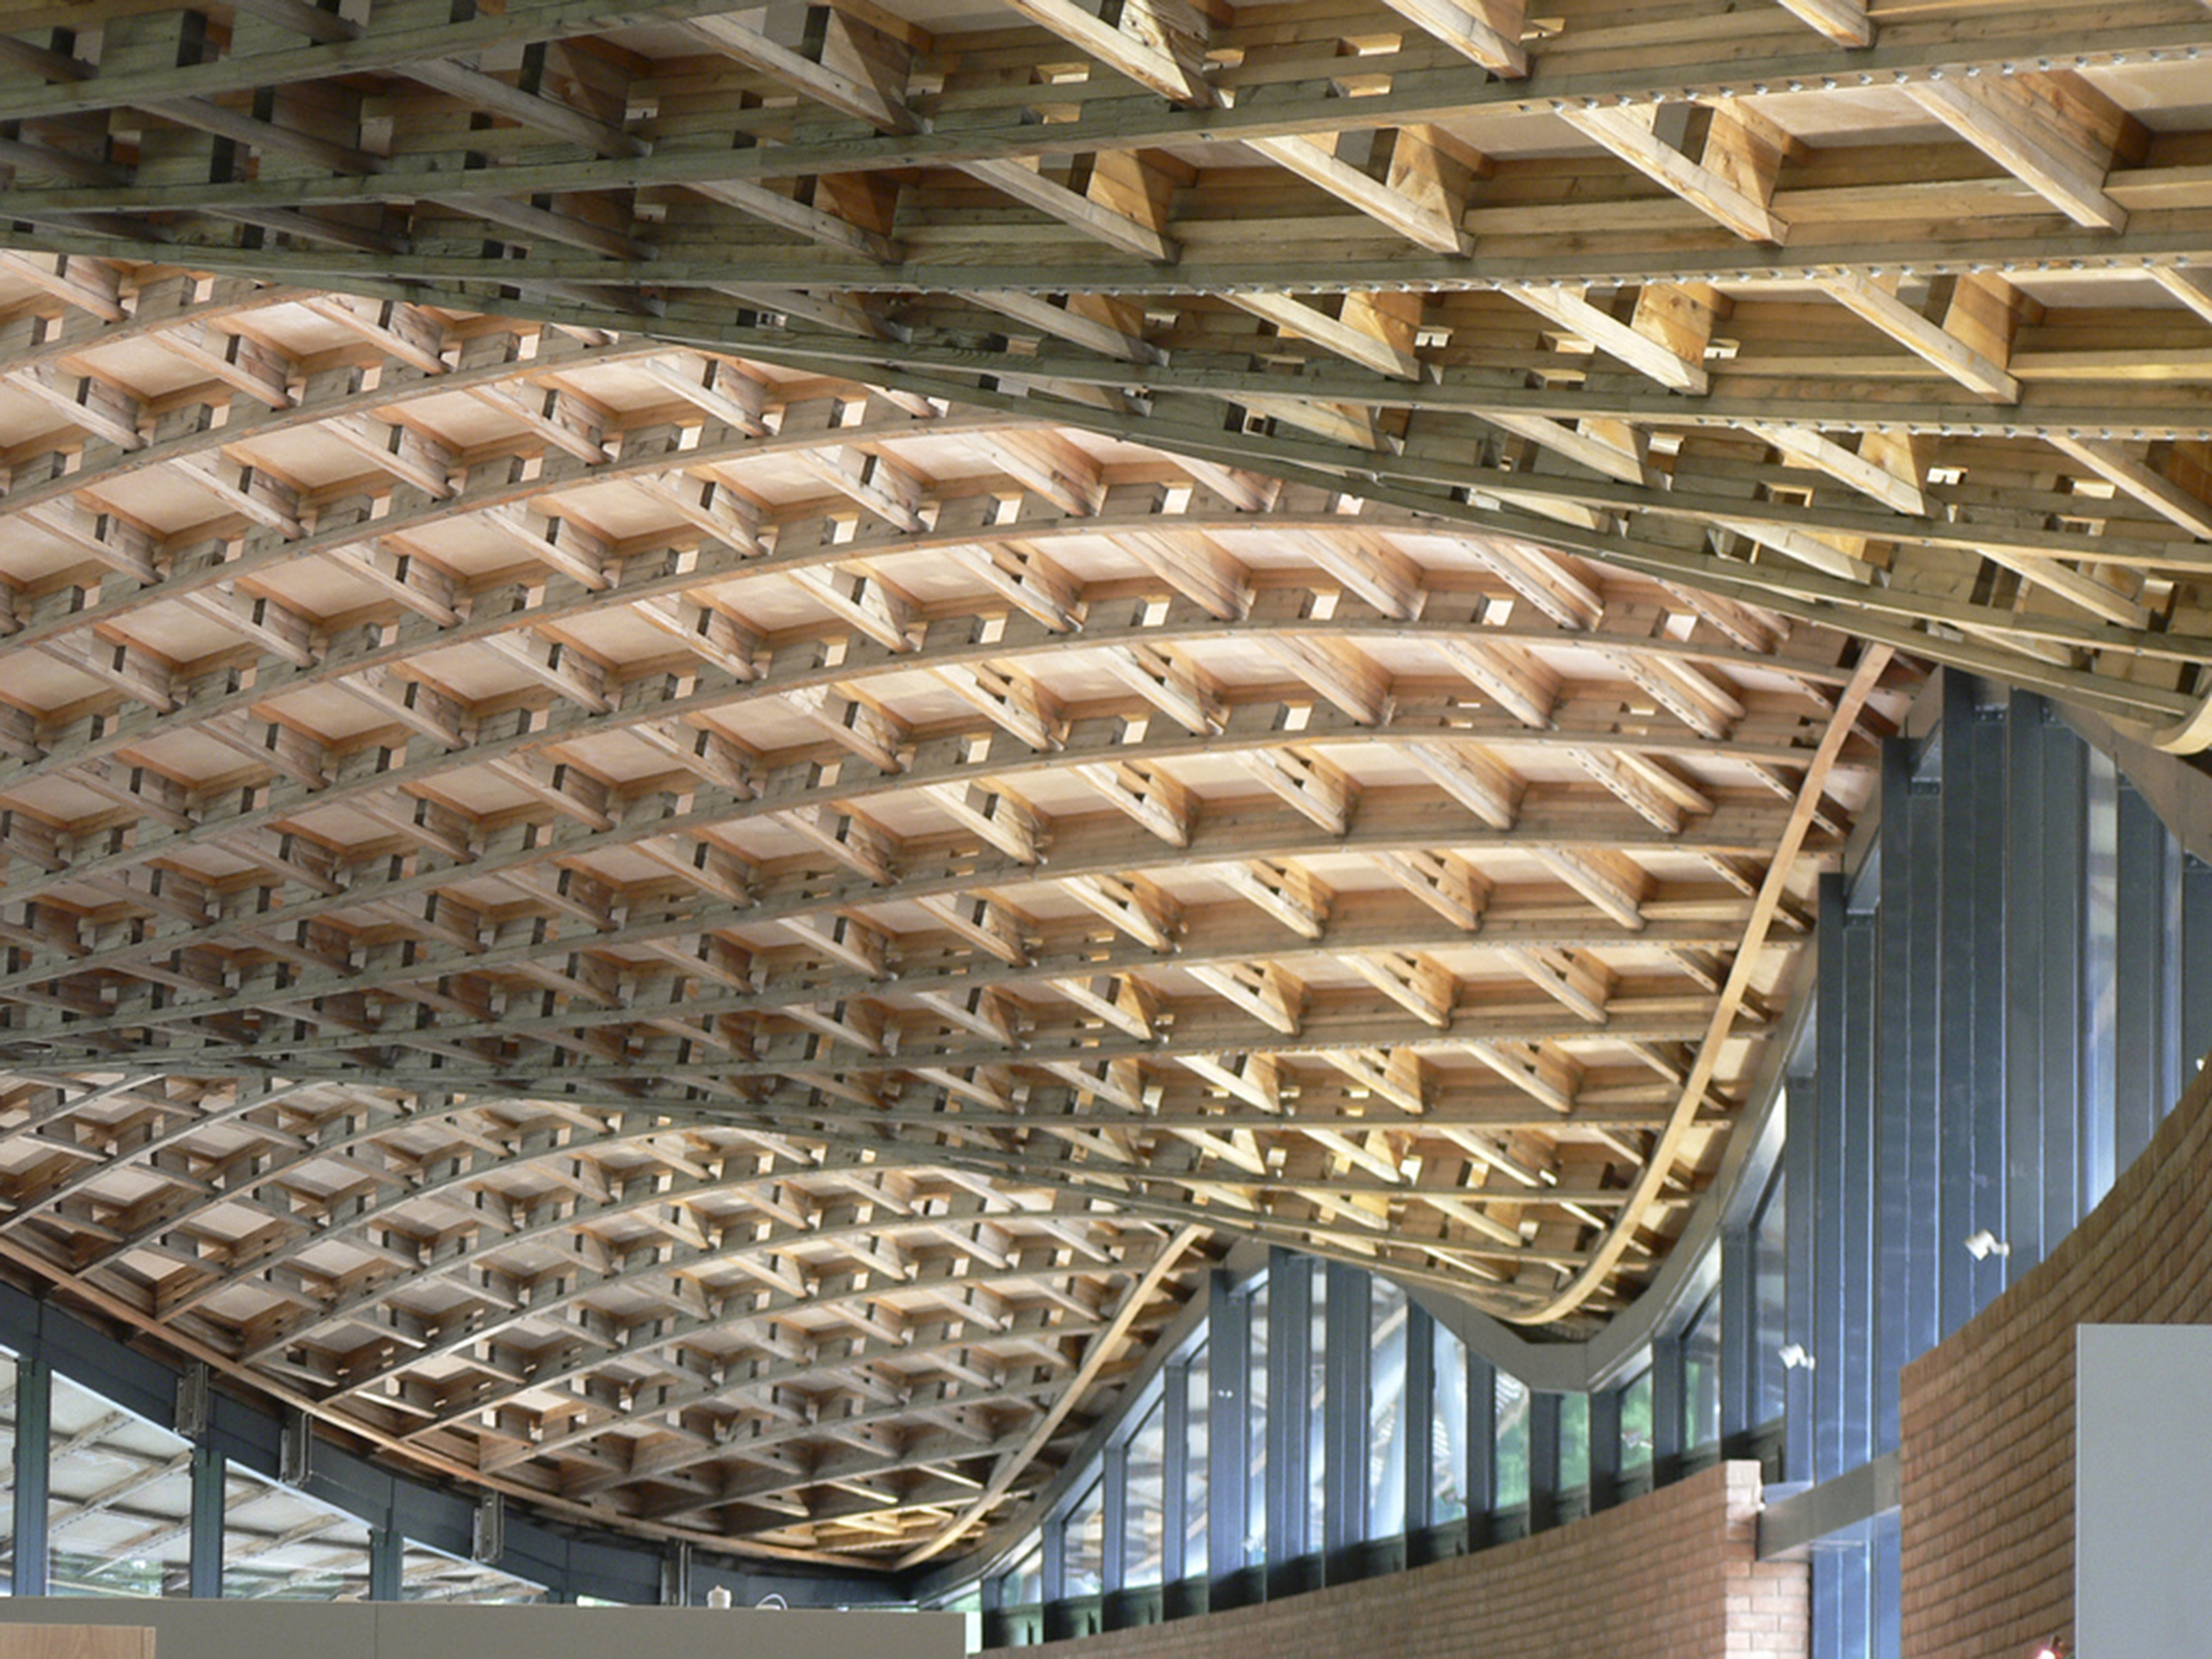
\includegraphics[width=0.5\paperwidth]{savill_b.jpg}
	% \end{textblock*}
	
	% full spread
	\cleartoleftpage
	\kant[1-2]	
	\PhotoSpread[lpcode=\mycap]{savill_a.jpg}

	% north west
	\cleartoleftpage
	\kant[1-2]	
	\PhotoSpread[width=1.5\paperwidth,xshift=1cm,yshift=-1cm,lpcode=\mycap]{savill_a.jpg}

	% south west
	\cleartoleftpage
	\kant[1-2]	
	\PhotoSpread[yanchor=south,width=1.5\paperwidth,xshift=1cm,yshift=1cm]{savill_a.jpg}

	% north east
	\cleartoleftpage
	\kant[1-2]	
	\PhotoSpread[lpstyle=plain,yanchor=north,xanchor=east,width=1.5\paperwidth,xshift=-1cm,yshift=-1cm]{savill_a.jpg}

	% south east
	\cleartoleftpage
	\kant[1-2]	
	\PhotoSpread[lpstyle=plain,yanchor=south,xanchor=east,width=1.5\paperwidth,xshift=-1cm,yshift=1cm]{savill_a.jpg}

	
\end{document}